The \code{sp} subcommand optimizes the location of sensors in a
water distribution network to minimize the impact of potential
contamination incidents. The \code{sp} subcommand has a rich interface
that supports a variety of optimization formulations, and it 
integrates a wide range of optimization solvers. 
An impact file is used to define the ensemble of contamination
incidents. By default, sensors can be placed at any feasible junction in
the network, but fixed and infeasible locations can be 
specified within the \code{sp} subcommand. 

A flowchart representation of the \code{sp} subcommand is shown in Figure \ref{fig:sp-flowchart}. 

\begin{figure}[h!]
  \centering
  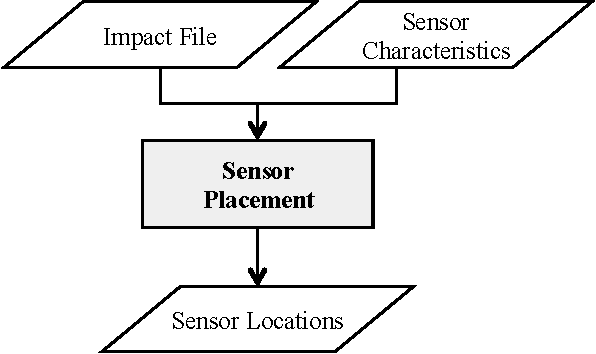
\includegraphics[scale=0.80]{graphics/sp_flowchart.pdf}
  \caption{Sensor placement flowchart.}
  \label{fig:sp-flowchart}
\end{figure}

The required input for the \code{sp} subcommand is an impact file and 
sensor characteristics. The impact file could be created by the \code{sim2Impact} subcommand,
or through some non-WST impact calculation process.
Multiple impact files can be used as input to the sensor placement problem. The other
required input is the sensor characteristics. These characteristics are supplied through
the \code{sp} WST configuration file as well as additional files that provide details 
on the cost and failure rates of the sensors.

Advanced features of the \code{sp} subcommand are discussed in
Section~\ref{chap:pmedian}. This includes a discussion of how to specify
feasible sensor locations and evaluation techniques. The section
also includes advanced sensor placement methods for computing a
bound on the quality of sensor networks, and techniques for minimizing
memory used during sensor placement: (a) aggregation of scenarios
and (b) skeletonization of the water distribution system network
model.



\section{Sensor Placement Formulations}\label{sp_formulation}

Several sensor placement optimization formulations are available
in the \code{sp} subcommand. The following formulations are described
below: expected-\/impact, robust optimization, side-constrained
and minimum cost formulations. WST also supports several sensor
placement formulations that are not documented yet: multi-stage
sensor placement and imperfect sensor models.

\subsection{Expected-\/Impact Formulation}\label{sp:average_formulation}

The most widely studied sensor placement formulation for a contamination warning system 
(CWS) design is to minimize the expected impact of an ensemble of contamination incidents 
given a fixed number of sensors. This formulation has also become the standard formulation 
in the \code{sp} subcommand, because it can be effectively used to select sensor placements 
in large water distribution networks.

A mixed-integer programming (MIP) formulation for expected-\/impact sensor placement is (eSP): 
\begin{align}
\textrm{minimize} \qquad & \sum_{a \in A} \alpha_a \sum_{i \in {\cal L}_a} d_{ai} x_{ai} \label{eqn:eSP} \\
\textrm{subject to} \qquad &\sum_{i\in {\cal L}_a} x_{ai} = 1 &&\forall a \in A\\ 
&x_{ai} \le s_i &&\forall a \in A, i \in {\cal L}_a\\  
&\sum_{i \in L} c_i s_i \le p\\ 
&s_i \in \{0,1\} &&\forall i \in L\\ 
&0 \leq x_{ai} \leq 1 &&\forall a \in A, i \in {\cal L}_a 
\end{align}

This MIP minimizes the expected impact of a set of contamination incidents defined by $A$. 
For each incident $a \in A$, $\alpha_a$ is the weight of incident $a$, which is typically a 
probability. This formulation integrates contamination impact calculations, which 
are reported at a set of locations from the full set, denoted $L$, 
where a location refers to a network node. For each incident $a$, ${\cal L}_a \subseteq L$ 
is the set of locations that can be contaminated by $a$. Thus, a sensor at a 
location $i \in {\cal L}_a$ can detect contamination from incident $a$ at the time 
contamination first arrives at location $i$. Each incident is witnessed 
by the first sensor to see it. For each incident $a \in A$ and location 
$i \in {\cal L}_a$, $d_{ai}$ defines the impact of the contamination incident $a$ 
if it is witnessed by location $i$. This impact metric assumes that as soon as a 
sensor witnesses contamination, then any further contamination impacts are mitigated 
(perhaps after a suitable delay that accounts for the response time of the water utility). 
The $s_i$ variables indicate where sensors are placed in the network, $c_i$ is 
the cost of placing a sensor at location $i$ and $p$ is the budget.

The $x_{ai}$ variables indicate whether incident $a$ is witnessed by a sensor at 
location $i$. They are defined as continuous variables between 0 and 1. 
In practice, there is always an optimal solution where $x_{ai}$ is binary. 
If $x_{ai}$ is fractional, then two or more equally good locations have sensors 
\citet{TEVASPOTCompendium10}. A given set of sensors might not be able to witness 
all contamination incidents. To account for this, $L$ contains a dummy location, $q$. 
The dummy location is assigned the impact if contamination was not detected at any node location. 
The dummy location is not a physical location in the network.
This dummy location is in all sets ${\cal L}_a$. If the dummy location witnesses
an incident, it generally means that no real sensor can detect that incident. The 
impact for this location is the impact of the contamination incident after the entire 
contaminant transport simulation has finished, which estimates the impact that 
would occur without an online sensor network. The impact of a dummy detection is greater
than all other impacts for each incident, so the witness variable $x_{ai}$ for the 
dummy will only be selected if no sensors have been placed that can detect this 
incident with smaller impact.

For examples on expected-\/impact sensor placement (eSP), see Example
\ref{sp_example1}, \ref{sp_example2} and \ref{sp_example3}.
\citet{BerHarPhiUbeWat06} describe eSP, and they note that this
formulation is identical to the well-\/known $p$-\/median facility
location problem \citep{MirFra90} when $c_i=1$. In the $p$-\/median
problem, $p$ facilities (e.g., central warehouses) are to be located
on $m$ potential sites such that the sum of distances $d_{ai}$
between each of $n$ customers (e.g., retail outlets) and the nearest
facility $i$ is minimized. In comparing eSP and $p$-\/median problems,
there is equivalence between (1) sensors and facilities, (2)
contamination incidents and customers and (3) contamination impacts
and distances. While eSP allows placement of at most $p$ sensors,
$p$-\/median formulations generally enforce placement of all $p$
facilities; in practice, the distinction is irrelevant unless $p$
approaches the number of possible locations. This equivalence enables the application of $p$-\/median 
solvers to eSP (see Example~\ref{sp_example3}).


\subsection{Robust Formulations}\label{sp:robust_formulation}

The eSP model described in Section \ref{sp:average_formulation} can
be viewed as optimizing one particular statistic of the distribution
of impacts defined by the contaminant transport simulations. However,
other statistics might provide more robust solutions that are 
less sensitive to changes in this distribution~\citep{WatHarMur06a, WatMurHar09}. 
Consider the following generalization of eSP:
\begin{align}
\textrm{minimize} \qquad &\textrm{Impact}_{f}(\alpha,d,x) \\
\textrm{subject to} \qquad &\sum_{i\in {\cal L}_a} x_{ai} = 1 &&\forall a \in A\\ 
&x_{ai} \le s_i &&\forall a \in A, i \in {\cal L}_a\\  
&\sum_{i \in L} c_i s_i \le p\\ 
&s_i \in \{0,1\} &&\forall i \in L\\ 
&0 \leq x_{ai} \leq 1 &&\forall a \in A, i \in {\cal L}_a 
\end{align}

The function $\textrm{Impact}_ {f}(\alpha,d,x)$ computes a statistic of the impact 
distribution. The following functions supported in WST have been developed by 
researchers to find robust solutions to optimization problems \citep{WatHarMur06a, WatMurHar09}:
\begin{itemize}
\item {\bfseries Mean:} This is the statistic used in eSP (Equation \ref{eqn:eSP})
\item {\bfseries VaR:} Value-\/at-\/Risk (VaR) is a percentile-\/based metric. 
Given a confidence level $\beta\in(0,1)$, the VaR is the value of the distribution 
at the $1-\beta$ percentile \citep{TopVlaZen02}. The value of VaR is less than 
the TCE value (see below).
Mathematically, suppose a random variable $W$ describes the distribution of possible 
impacts. The probability that $W$ is less than a value $w$ is denoted as $\P[W \le w]$. Then 
\begin{equation}
{\rm VaR}(W,\beta) = \min \{ w \mid \P[W \le w] \ge \beta \} 
\end{equation}
Note that the distribution $W$ changes with each sensor placement. Further, VaR 
can be computed using the $\alpha$, $d$ and $x$ values.
\item {\bfseries TCE:} The Tail-\/Conditioned Expectation (TCE) is a related 
metric that measures the conditional expectation of impact exceeding VaR at a 
given confidence level. Given a confidence level $1-\beta$, TCE is the expectation 
of the worst impacts whose likelihood sums to $\beta$. This value is between VaR and 
the worst-\/case value.
Mathematically, then
\begin{equation}
{\rm TCE}(\beta) = {\rm E}\left[ W \mid W \ge {\rm VaR}(\beta) \right]
\end{equation}
\item {\bfseries CVar:} The Conditional Value-\/at-\/Risk (CVaR) is a 
linearization of TCE investigated by \citet{rockafellar02cvar}. CVaR 
approximates TCE with a continuous, piecewise-\/linear function of $\beta$, 
which enables the use of CVaR in a MIP model.
\item {\bfseries Worst:} The worst impact value can be easily computed, since a 
finite number of contamination incidents are simulated. However, this statistic 
is sensitive to changes in the number of contamination incidents that are simulated; 
adding additional contamination incidents could significantly impact this statistic.
\end{itemize}

WST includes robust MIP reformulations of eSP for the the worst and CVar statistics. 
The reformulation to minimize the worst contamination impact is (wSP):
\begin{align}
\textrm{minimize} \qquad & w \label{eqn:wSP} \\
\textrm{subject to} \qquad & \alpha_a \sum_{i \in {\cal L}_a} d_{ai} x_{ai} \leq w && \forall a \in A\\
&\sum_{i\in {\cal L}_a} x_{ai} = 1 &&\forall a \in A\\ 
&x_{ai} \le s_i &&\forall a \in A, i \in {\cal L}_a\\  
&\sum_{i \in L} c_i s_i \le p\\ 
&s_i \in \{0,1\} &&\forall i \in L\\ 
&0 \leq x_{ai} \leq 1 &&\forall a \in A, i \in {\cal L}_a 
\end{align}
This is a standard formulation for the $p$-\/center problem \citep{Daskin95,ElloumiEtAl04}.

Similarly, the reformulation to minimize CVaR is (cvarSP):
\begin{align}
\textrm{minimize} \qquad & v + \frac{1}{\beta} \sum_{a \in A} \alpha_a y_a \label{eqn:cvarSP} \\
\textrm{subject to} \qquad & y_a \geq \sum_{i \in {\cal L}_a} d_{ai} x_{ai} - v && \forall a \in A\\
&y_q \geq 0 &&\forall a \in A \\
&\sum_{i\in {\cal L}_a} x_{ai} = 1 &&\forall a \in A\\ 
&x_{ai} \le s_i &&\forall a \in A, i \in {\cal L}_a\\  
&\sum_{i \in L} c_i s_i \le p\\ 
&s_i \in \{0,1\} &&\forall i \in L\\ 
&0 \leq x_{ai} \leq 1 &&\forall a \in A, i \in {\cal L}_a 
\end{align}
The variable $v$ represents $\rm VaR$, which is implicitly computed when this model is solved.
See \citet{rockafellar02cvar} for further discussion of CVaR formulations.

Note that these formulations share a core set of constraints and
variables with eSP. The difference in these models is how the
objective is expressed.
For examples on robust sensor placement (wSP and cvarSP), see Example \ref{sp_example4} and \ref{sp_example5}.


\subsection{Side-\/Constrained Formulation}\label{sp:sc_formulation}

Another natural generalization of eSP is to consider the addition
of side constraints that represent bounds on alternate objectives
or statistics. For example, consider a simple extension of eSP that
includes a single side-constraint (scSP):
\begin{align}
\textrm{minimize} \qquad & \sum_{a \in A} \alpha_a \sum_{i \in {\cal L}_a} d_{ai} x_{ai} \label{eqn:scSP} \\
\textrm{subject to} \qquad &\sum_{i\in {\cal L}_a} x_{ai} = 1 &&\forall a \in A\\ 
&x_{ai} \le s_i &&\forall a \in A, i \in {\cal L}_a\\  
&\sum_{i \in L} c_i s_i \le p\\ 
&s_i \in \{0,1\} &&\forall i \in L\\ 
&0 \leq x_{ai} \leq 1 &&\forall a \in A, i \in {\cal L}_a\\
& \sum_{a \in A} \alpha_a \sum_{i \in {\cal L}_a} \hat{d}_{ai} x_{ai} \leq G
\end{align}

The last constraint in this formulation bounds the value of an
impact statistic $\hat{d}_{ai}$. Note that this statistic could 
easily be used as the objective for (eSP). This can be
viewed as a goal constraint. Iteratively solving scSP for different
goals, $G$, provides an assessment of the trade-off between the impact
statistics in the objective and this constraint. Hence, the scSP formulation
provides a mechanism for analyzing trade-\/offs between different objectives.

WST provides general support for side-constraints beyond what is
represented in scSP, since multiple side-constraints can
be specified. Additionally, robust statistics can be specified.
For example, WST can express sensor placement formulations where
the mean impact is minimized while the worst-case impact is
constrained.
See Example \ref{sp_example6} for a demonstration of side-\/constrained sensor placement (scSP).


\subsection{Min-\/Cost Formulation}\label{sp:minCost_formulation}

The eSP model described in Section~\ref{sp:average_formulation}
minimizes expected contamination impact subject to a cost constraint
on the number of sensors that are installed. A related sensor
placement formulation is to minimize the cost of installing sensors
while constraining the contamination impact to be below a specified
threshold, $u$. 

For example, eSP can be reformulated to minimize cost (mcSP):
\begin{align}
\textrm{minimize} \qquad & \sum_{i \in L} c_i s_i \label{eqn:ceSP} \\
\textrm{subject to} \qquad &\sum_{i\in {\cal L}_a} x_{ai} = 1 &&\forall a \in A\\ 
&x_{ai} \le s_i &&\forall a \in A, i \in {\cal L}_a\\  
&\sum_{a \in A} \alpha_a \sum_{i \in {\cal L}_a} d_{ai} x_{ai} \leq u\\
&s_i \in \{0,1\} &&\forall i \in L\\ 
&0 \leq x_{ai} \leq 1 &&\forall a \in A, i \in {\cal L}_a 
\end{align}

See Example \ref{sp_example7} for a demonstration of min-\/cost sensor placement (mcSP).

\if 0
\subsection{Multiple Objective Formulation}\label{sp:multiObj_formulation}

CWS design generally requires the evaluation and optimization of a variety of 
performance objectives. Some performance objectives cannot be simultaneously optimized, 
and thus a CWS design must be selected from a trade-\/off between these   
objectives~\cite{WatGreHar04a}.

The \code{sp} subcommand supports the analysis of these trade-\/offs with the specification of additional 
constraints on impact measures. For example, a user can minimize the expected 
extent of contamination (EC) while constraining the worst-\/case time to 
detection (TD). The \code{sp} subcommand allows for the specification of more than one impact 
constraint. However, the sensor placement solvers cannot reliably optimize formulations with 
more than one impact constraint.

\subsection{Imperfect Sensors Formulation}\label{sp:imperfect_formulation}

The previous sensor placement formulations make the implicit assumption that 
sensors work perfectly. That is, they never fail to detect a contaminant when it 
exists, and they never generate an erroneous detection when no contaminant exists. 
In practice, sensors are imperfect, and they generate these types of errors.

The \code{sp} subcommand addresses this issue by supporting a formulation that models simple sensor 
failures~\cite{BerryCHLPW09}. Each sensor, $s_i$, has an associated probability
of failure, $p_i$. With these probabilities, the probability 
that a contamination incident will be detected by a particular sensor can be easily assessed. Thus, it 
is straightforward to compute the expected impact of a contamination incident.

This formulation does not explicitly allow for the specification of probabilities 
of false detections. These probabilities do not impact the performance of a CWS 
during a contamination incident. Instead, they impact the day-\/to-\/day maintenance
and use of the CWS; erroneous detections create work for the CWS users, which is an 
ongoing cost. The overall likelihood of false detections is simply a function of the
sensors that are selected. In cases where every sensor has the same likelihoods, this 
implies a simple constraint on the number of sensors. 
\fi

\section{Sensor Placement Solvers}

The \code{sp} subcommand performs optimization using a solver specified in the
configuration file. All of the solvers supported by the \code{sp} subcommand are practical
for small-\/sized water distribution networks, and heuristic
solvers can be used to find sensor placements for very large networks.

The \code{sp} subcommand interfaces with a variety of external
solvers that can be used to perform sensor placement. Several
different MIP solvers can be used to find a globally optimal solution
for the eSP MIP formulation. However, this might be a computationally
expensive process (especially for large problems), and the size of
the MIP formulation can become prohibitively large in some cases. 
A variety of public-domain and commercial solvers can be used by
the \code{sp} subcommand, including GLPK, CBC, PICO, CPLEX, GUROBI and
XPRESS.

% TODO - verify this text.  How do we name these solvers?

A greedy randomized adaptive sampling process (GRASP) heuristic 
performs sensor placement optimization without
explicitly creating a MIP formulation. Thus, this solver uses much
less memory, and it usually runs very quickly. Although the GRASP
heuristic does not guarantee that a globally optimal solution is
found, it has proven effective at finding optimal solutions to a
variety of large-scale applications. Two different implementations
of the GRASP solvers can be used: an AT\&T commercial solver (att\_grasp)
or an open-source implementation of this solver (snl\_grasp).

% TODO - verify this text.  What is the status of this solver?

The Lagrangian heuristic uses the structure of the $p$-\/median MIP
formulation (eSP) to find near-optimal solutions while computing a
lower bound on the best possible solution.


\section{\code{sp} Subcommand}

The \code{sp} subcommand is executed with the following command:

\begin{unknownListing}
wst sp <configfile>
\end{unknownListing}

where \code{configfile} is a WST configuration file in the YAML format. 

The \code{---help} option prints information about this subcommand, such as usage,
arguments and a brief description:

\begin{unknownListing}
wst sp --help
\end{unknownListing}

Two other options can be used to print help information. 
The \code{---help-problems} option prints a table of the different types of 
optimization problems that can be solved with the \code{sp} subcommand. For example, 
the following is a description of the standard problem solved by the \code{sp} subcommand (eSP):

\begin{unknownListing}
default, p-median, average-case perfect-sensor
---------------------------------------------- 
mean obj
0 constraints
perfect
single obj
1 stage
exact
\end{unknownListing}

The first row lists the different names that can be used to specify
this problem type. These are synonyms, since the standard problem,
eSP, is a $p$-\/median problem where the objective is an average statistic.
This is also the standard perfect-sensor formulation, where all
sensors are assumed to work perfectly without failures.
The six rows following the dashed lines are different characteristics of this problem: 
\begin{enumerate}
\item the type of objective used
\item the number of side-constraints
\item specify whether sensors are perfect (i.e., without failures) or whether they can fail
\item the number of objectives
\item the number of stages (i.e., time steps) in the sensor placement formulation
\item the type of solution that is required (e.g., an exact solution versus any feasible solution).
\end{enumerate}
These six characteristics are used by the \code{sp} subcommand 
to verify the suitability of solvers that are specified for optimization.

The \code{---help-solvers} option prints a table of the different solvers that can
be applied to perform optimization. For example, the following is a description
of the solvers that can be used to optimize \code{average-case perfect-sensor} problems (which is the default):

\begin{unknownListing}
Problem Type                  Solver        Modeling Language  
======================================================================
average-case perfect-sensor   *att_grasp     none               
average-case perfect-sensor   *cbc           pyomo              
average-case perfect-sensor   *cplex         pyomo              
average-case perfect-sensor   *glpk          pyomo              
average-case perfect-sensor    gurobi        pyomo              
average-case perfect-sensor   *lagrangian    none               
average-case perfect-sensor    pico          ampl               
average-case perfect-sensor    pico          pyomo              
average-case perfect-sensor   *snl_grasp     none               
average-case perfect-sensor    xpress        pyomo     
\end{unknownListing}

Solvers highlighted with an asterisk are available in the current
installation of WST. The modeling language indicates whether AMPL
\citep{AMPL}, Pyomo \citep{PYOMO} or neither is used to solve sensor
placement optimization problem. Note that GLPK includes a modeling
tool that includes a subset of AMPL. Thus, problems that require
AMPL can be solved if either AMPL or GLPK is installed.


\subsection{Configuration File}

The \code{sp} subcommand generates a template configuration file using the following command line:
\begin{unknownListing}
wst sp --template <configfile>
\end{unknownListing}

The template configuration file for the \code{sp} subcommand is shown in Figure \ref{fig:sp_template}.  
Brief descriptions of the options are included in the template after the \# character.  

\begin{figure}[h!]
	\unknownInputListing{examples/sp_config.yml}{}{1}{24}
	\caption[The \code{sp} configuration template file]{The \code{sp} configuration template file (\textit{continued in Figure \ref{fig:sp_template_ctd}}).}
	\label{fig:sp_template}
\end{figure}

\begin{figure}[h!]
	\unknownInputListing{examples/sp_config.yml}{}{25}{67}
	\caption[The \code{sp} configuration template file (ctd.)]{The \code{sp} configuration template file (\textit{continued from Figure \ref{fig:sp_template}}).}
	\label{fig:sp_template_ctd}
\end{figure}

\clearpage
\subsection{Configuration Options}

Full descriptions of the WST configuration options used by the \code{sp} subcommand are listed below.
\begin{description}[topsep=0pt,parsep=0.5em,itemsep=-0.4em]
  \item[{impact data}]\hfill
  \begin{description}[topsep=0pt,parsep=0.5em,itemsep=-0.4em]
    \item[{name}]\hfill
\\The name of the impact block that is used in the objective or constraint block.
                
                Required input.
                
    \item[{impact file}]\hfill
\\The name of the impact file that is created by \code{sim2Impact} and 
                contains the detection time and the total
                impact given a sensor at that node is the first to detect
                contamination from that scenario. 
                The impact file format is documented in File Formats Section \ref{formats_impactFile}.
                
                Required input.
                
    \item[{nodemap file}]\hfill
\\The name of the nodemap file that is created by \code{sim2Impact} and 
                maps sensor placement ids to the network node labels. 
                The nodemap file format is documented in File Formats Section \ref{formats_nodeFile}.
                
                Required input.
                
    \item[{weight file}]\hfill
\\The name of the weight file that specifies the weights for contamination
                incidents. This file supports the optimization of weighted
                impact metrics. 
                The weight file format is documented in File Formats Section \ref{formats_weightFile}.
                
                Optional input; by default, incidents are optimized with weight 1.
  \end{description}

  \item[{cost}]\hfill
  \begin{description}[topsep=0pt,parsep=0.5em,itemsep=-0.4em]
    \item[{name}]\hfill
\\The name of the cost block that is used in the objective or constraint block.
                
                Optional input.
    \item[{cost file}]\hfill
\\The name of the cost file that contains the costs for the installation of
                sensors throughout the distribution network. This file contains
                EPANET ID/cost pairs.
                The cost file format is documented in File Formats Section \ref{formats_costFile}.
                
                Optional input.
  \end{description}
  \item[{objective}]\hfill
  \begin{description}[topsep=0pt,parsep=0.5em,itemsep=-0.4em]
    \item[{name}]\hfill
\\The name of the objective block that is used in sensor placement block.
                
                Required input.
    \item[{goal}]\hfill
\\The objective of the optimization process that defines what is going to minimized. 
                The options are the name of the impact block, the name of the cost block, 
                the number of sensors (NS) or the number of failed detections (NFD).
				
				Required input.
    \item[{statistic}]\hfill
      \\The objective statistic. The TOTAL
      statistic is used when the goal is NS                             or
      NFD. When the goal is to compute a                             statistic
      of an impact block, the options                             are MEAN,
      MEDIAN, VAR, TCE, CVAR, TOTAL                             or WORST. For
      example, MEAN will minimize                             the mean impacts
      over all of the                             contamination scenarios,
      while WORST                             will only minimize the worst
      impacts                             from the ensemble of contamination
      scenarios.                                  Required input.
    \item[{gamma}]\hfill
      \\The value of gamma that specifies the                 fraction of the
      distribution of impacts that will                 be used to compute the
      VAR, CVAR and TCE statistics.                 Gamma is assumed to be in
      the interval (0,1], which means                  that gamma can be
      greater than zero but less than or equal to one. It                 can
      be interpreted as specifying the 100*gamma                 percent of
      the worst contamination incidents that                 are used for
      these calculations.                  Required input for VAR or CVAR
      objective statistics,                 default = 0.05.
  \end{description}
  \item[{constraint}]\hfill
  \begin{description}[topsep=0pt,parsep=0.5em,itemsep=-0.4em]
    \item[{name}]\hfill
\\The name of the constraint block that is used in sensor placement block.
                
                Required input.
    \item[{goal}]\hfill
\\The constraint goal. The options are the name of the impact block name, 
                the name of the cost block, the number of sensors (NS) or the number of failed detections (NFD).
                
                Required input.
    \item[{statistic}]\hfill
\\The constraint statistic. The TOTAL
                statistic is used when the goal is NS
                or NFD. When the goal is to compute a
                statistic of an impact block, the options
                are MEAN, MEDIAN, VAR, TCE, CVAR, TOTAL
                or WORST. For example, MEAN will constrain
                the mean impacts over all of the
                contamination scenarios, while WORST
                will only constrain the worst impacts
                from the ensemble of contamination
                scenarios.

                Required input.
    \item[{gamma}]\hfill
\\The value of gamma that specifies the fraction of the distribution of impacts that
                will be used to compute the VAR, CVAR and TCE statistics. Gamma
                is assumed to be in the interval (0,1], which means that gamma 
				can be greater than zero but less than or equal to one. It can be interpreted
                as specifying the 100*gamma percent of the worst contamination
                incidents that are used for these calculations.  
                
                Required input for VAR or CVAR objective statistics, default = 0.05.
    \item[{bound}]\hfill
\\The upper bound on the constraint.
                
                Optional input.
  \end{description}
  \item[{aggregate}]\hfill
  \begin{description}[topsep=0pt,parsep=0.5em,itemsep=-0.4em]
    \item[{name}]\hfill
\\The name of the aggregation block that is used in sensor placement block.
                
                Optional input.
    \item[{type}]\hfill
\\The type of aggregation used to reduce the size of the sensor placement problem.  
                The options are THRESHOLD, PERCENT or RATIO.

                THRESHOLD is used to aggregate similar impacts by specifying a goal and a value.  
                This is used to reduce the total size of the sensor placement formulation (for large problems).
                Solutions generated with non-zero thresholds are not guaranteed
                to be globally optimal.

                PERCENT is an alternative method to compute the aggregation threshold 
                in which the value (of the goal-value pair) is a real number between 0.0 and 1.0. 
                Over all contamination incidents, compute the maximum difference, d, between the impact of the
                contamination incident if it is not detected and the impact if it is detected
                at the earliest possible feasible location and set the aggregation threshold to 
                d times the aggregation percent. If both THRESHOLD and PERCENT are set to valid values, 
                then PERCENT takes priority.

                RATIO is also specified with a goal-value pair in which value is a real number between
                0.0 and 1.0.
                
                Optional input.
    \item[{goal}]\hfill
\\The aggregation goal for the aggregation type.
                
                Optional input.
    \item[{value}]\hfill
\\The aggregation value for the aggregation type. If the aggregation type is PERCENT or RATIO,
                then this value is a real number between 0.0 and 1.0.
                
                Optional input.
    \item[{conserve memory}]\hfill
\\The maximum number of impact files that should be read into memory 
                at any one time. This option allows impact files to be processed in 
                a memory conserving mode if location aggregation is chosen and the original impact
                files are very large. For example, a conserve memory value of 10000 requests
                that no more than 10000 impacts should be read into memory at any one 
                time while the original impact files are being processed into smaller
                aggregated files.  
				
				Optional input, default = zero to turn off this option.
    \item[{distinguish detection}]\hfill
\\A goal for which aggregation should not allow incidents to
                become trivial. If the aggregation threshold is so large that all
                locations, including the dummy, would form a single superlocation,
                this forces the dummy to be in a superlocation by itself. Thus,
                the sensor placement will distinguish between detecting and not
                detecting. This option can be listed multiple times, to specify
                multiple goals. 
                
                Optional input, default = 0.
    \item[{disable aggregation}]\hfill
\\Disable aggregation for this goal, even at value zero, which
                would incur no error. Each witness incident will be in a separate
                superlocation. This option can be listed multiple times to
                specify multiple goals. ALL can be used to specify
                all goals. 
                
                Optional input, default = 0.
  \end{description}
  \item[{imperfect}]\hfill
  \begin{description}[topsep=0pt,parsep=0.5em,itemsep=-0.4em]
    \item[{name}]\hfill
\\The name of the imperfect block that is used in sensor placement block.
                
                Optional input.
    \item[{sensor class file}]\hfill
\\The name of the imperfect sensor class file that defines the detection probabilities
                for all sensor categories. It is used with the imperfect-sensor model 
                and must be specified in conjunction with a imperfect junction class file.
                The imperfect sensor class file format is documented in File Formats Section \ref{formats_sensorClass}.
                
                Optional input.
    \item[{junction class file}]\hfill
\\The name of the imperfect junction class file that defines a sensor category for
                each network node. It is used with the imperfect-sensor model and
                must be specified in conjunction with a imperfect sensor class file.
                The imperfect junction class file format is documented in File Formats Section \ref{formats_junctionClass}.
                
                Optional input.
  \end{description}
  \item[{sensor placement}]\hfill
  \begin{description}[topsep=0pt,parsep=0.5em,itemsep=-0.4em]
    \item[{type}]\hfill
\\The sensor placement problem type. The command \code{wst sp ---help-problems} 
                provides a list of problem types for sensor placement. For example, average-case perfect-sensor
                is the standard problem type for sensor placement, since it uses the mean statistic, 
                zero constraints, single objective and perfect sensors. 
                
                Required option, default = average-case perfect-sensor.
    \item[{modeling language}]\hfill
\\The modeling language to generate the sensor placement optimization 
                problem. The options are NONE, PYOMO or AMPL. 

                Required input, default = NONE.
    \item[{objective}]\hfill
\\The name of the objective block previously defined to be used in sensor placement.
                
                Required input.
    \item[{constraint}]\hfill
\\The name of the constraint block previously defined to be used in sensor placement.
                
                Required input.
    \item[{imperfect}]\hfill
\\The name of the imperfect block previously defined to be used in sensor placement.
                
                Optional input.
    \item[{aggregate}]\hfill
\\The name of the aggregate block previously defined to be used in sensor placement.
                
                Optional input.
    \item[{compute bound}]\hfill
\\A flag to indicate if bounds should be computed on the sensor placement
                solution. The options are true or false. 
                
                Optional input, default = false.
    \item[{presolve}]\hfill
\\A flag to indicate if the sensor placement problem should be presolved. 
                The options are true or false. 
                
                Optional input, default = true.
    \item[{compute greedy ranking}]\hfill
\\A flag to indicate if a greedy ranking of the sensor locations should be calculated. 
                The options are true or false. 
                
                Optional input, default = false.
    \item[{location}]\hfill
    \begin{description}[topsep=0pt,parsep=0.5em,itemsep=-0.4em]
      \item[{feasible nodes}]\hfill
\\A list that defines nodes that can be considered for the sensor placement problem.
                The options are:
                (1) ALL, which specifies all nodes as feasible sensor locations;
                (2) NZD, which specifies all non-zero demand nodes as feasible sensor locations;
                (3) a list of EPANET node IDs, which identifies specific nodes as feasible sensor locations; 
                (4) a filename, which references a space or comma separated file containing a list of 
                specific nodes as feasible sensor locations; or
                (5) NONE, which indicates this option is ignored.
                
                Required input, default = ALL.
      \item[{infeasible nodes}]\hfill
\\A list that defines nodes that cannot be considered for the sensor placement problem.
                The options are:
                (1) ALL, which specifies all nodes as infeasible sensor locations;
                (2) NZD, which specifies non-zero demand nodes as infeasible sensor locations;
                (3) a list of EPANET node IDs, which identifies specific nodes as infeasible sensor locations;
                (4) a filename, which references a space or comma separated file containing a list of 
                specific nodes as infeasible sensor locations; or
                (5) NONE, which indicates this option is ignored.
                
                Optional input, default = NONE.
      \item[{fixed nodes}]\hfill
\\A list that defines nodes that are already sensor locations.
                The options are:
                (1) ALL, which specifies all nodes as fixed sensor locations;
                (2) NZD, which specifies non-zero demand nodes as fixed sensor locations;
                (3) a list of EPANET node IDs, which identifies specific nodes as fixed sensor locations; 
                (4) a filename, which references a space or comma separated file containing a list of 
                specific nodes as fixed sensor locations; or
                (5) NONE, which indicates this option is ignored.
                
                Optional input, default = NONE.
      \item[{unfixed nodes}]\hfill
\\A list that defines nodes that are unfixed sensor locations.
                The options are:
                (1) ALL, which specifies all nodes as unfixed sensor locations;
                (2) NZD, which specifies non-zero demand nodes as unfixed sensor locations;
                (3) a list of EPANET node IDs, which identifies specific nodes as unfixed sensor locations; 
                (4) a filename, which references a space or comma separated file containing a list of 
                specific nodes as unfixed sensor locations; or
                (5) NONE, which indicates this option is ignored.
                
                Optional input, default = NONE.
    \end{description}
  \end{description}
  \item[{solver}]\hfill
  \begin{description}[topsep=0pt,parsep=0.5em,itemsep=-0.4em]
    \item[{type}]\hfill
\\The solver type. Each component of WST
				(e.g., sensor placement, flushing response, booster 
				placement) has different 
				solvers available. More specific details are provided in 
				the subcommand's chapter.
                
                Required input.
    \item[{options}]\hfill
\\A list of options associated with a specific solver type. More
            information on the options available for a specific solver
            is provided in the solver's documentation. The Getting
            Started Section \ref{dependencies} provides links to the
            different solvers.
            
            Optional input.
    \item[{threads}]\hfill
\\The maximum number of threads or function evaluations the solver is
                allowed to use.  This option is not available to all solvers or all analyses.
                
                Optional input.
    \item[{logfile}]\hfill
\\The name of a file to output the results of the solver.
                
                Optional input.
    \item[{verbose}]\hfill
\\The solver verbosity level.
                
                Optional input, default = 0 (lowest level).
    \item[{initial points}]\hfill
    \begin{description}[topsep=0pt,parsep=0.5em,itemsep=-0.4em]
      \item[{nodes}]\hfill
\\A list of node locations (EPANET IDs) to begin the optimization
        process. Currently, this option is only supported for the
        network solver used in the flushing and booster\_msx
        subcommands. This input causes an error for other subcommands.
        
        Optional input.
      \item[{pipes}]\hfill
\\A list of pipe locations (EPANET IDs) to begin the optimization
        process. Currently, this option is only supported for the
        network solver used in the flushing subcommand. This input causes an error for other subcommands.
        
        Optional input.
    \end{description}
  \end{description}
  \item[{configure}]\hfill
  \begin{description}[topsep=0pt,parsep=0.5em,itemsep=-0.4em]
    \item[{output prefix}]\hfill
\\The prefix used for all output files.
                
                Required input.
    \item[{output directory}]\hfill
      \\The output directory to store the results.
    \item[{debug}]\hfill
\\The debugging level (0 or 1) that indicates the amount of debugging 
                information printed to the screen, log file and output yml file. 
                
                Optional input, default = 0 (lowest level).
  \end{description}
\end{description}


\subsection{Subcommand Output}

The \code{sp} subcommand creates several output files.
The YAML file called <output prefix>sp\_output.yml contains the sensor locations,
final impact metric, the run date and CPU time. For some solvers, the
lower and upper bound on the objective is reported.   
The log file called <output prefix>sp\_output.log contains basic debugging information. 
A visualization YAML configuration file called
<output prefix>sp\_output\_vis.yml is also created and can be used to generate 
network graphics of the sensor placement solution using the \code{visualization} 
subcommand. The correct EPANET INP file must be included in the visualization YAML configuration 
file for the graphic to display properly.

The \code{sp} subcommand also outputs information a file named <output prefix>\_evalsensor.out 
That file includes the following data:
\begin{itemize}
\item {\bfseries Objective:} The impact metric value achieved with the sensor network design.
\item {\bfseries Lower bound:} The lower bound on the impact metric with the sensor network design.
\item {\bfseries Upper bound:} The upper bound on the impact metric with the sensor network design.
\item {\bfseries Solutions:} The internal node indices used by \code{sp} for the sensor network design.
\item {\bfseries Locations:} The EPANET junction labels for the sensor placement locations.
\item {\bfseries Sensor placement ID:} An integer ID used to distinguish the sensor network design.
\item {\bfseries Number of sensors:} The number of sensors in the sensor network design.
\item {\bfseries Total cost:} The cost of the sensor network design, which could be non-zero if cost data is provided.
\item {\bfseries Sensor node IDs:} The internal node indices used by \code{sp} for the sensor network design. The same as Solutions.
\item {\bfseries Sensor junctions:} The EPANET junction labels for the sensor placement locations. The same as Locations.
\item {\bfseries Impact file:} The name of the impact file used in the sensor network design.
\item {\bfseries Number of events:} The number of contamination scenarios that were simulated.
\end{itemize}

The performance of the sensor network design is summarized for each impact data file 
specified in the configuration file. The impact statistics included are: 
\begin{itemize}
\item {\bfseries Min impact:} The minimum impact over all contamination
incidents simulated. Assuming that a sensor protects the node
at which it is placed, this statistic will typically be zero.
\item {\bfseries Mean impact:} The mean (or average) impact over all
contamination incidents simulated.
\item {\bfseries Lower quartile impact:} 25\% of the contamination incidents,
weighted by their likelihood, have an impact value less than this quartile.
\item {\bfseries Median impact:} 50\% of the contamination incidents simulated, weighted
by their likelihood, have an impact value less than this quartile.
\item {\bfseries Upper quartile impact:} 75\% of the contamination incidents simulated,
weighted by their likelihood, have an impact value less than this quartile.
\item {\bfseries Value at Risk (VaR):} VaR is the minimum value
for which $100\times(1-\beta)$\% of the contamination incidents simulated have a smaller
impact, in which $\beta$ is a user-defined percentage between $ 0.0 < \beta < 1.0$.
\item {\bfseries TCE:} The tailed-\/conditioned expectation (TCE)
is the mean value of the impacts that are greater than or equal to VaR.
\item {\bfseries Worst impact:} The worst impact over all contamination
incidents simulated.
\end{itemize}

If the \code{[compute greedy ranking]} option is used, a greedy sensor placement is printed 
to <output prefix>\_evalsensor.out. The greedy ranking places sensors one-\/at-\/a-\/time at the locations 
in the optimal sensor network design by consecutively minimizing the mean impact 
of placing each sensor. This analysis gives a sense of the relative priorities for these
sensors. The greedy ranking is listed in terms of the sensor node IDs used by the 
\code{sp} subcommand. The corresponding EPANET node ID is listed at the top of the file.

\section{Sensor Placement Examples}\label{sp_example}

The following examples illustrate common ways that the \code{sp} subcommand can be used. 
Additional examples using the \code{sp} subcommand are provided in Section~\ref{chap:pmedian}.

\subsection{Example 1: Solving eSP with a MIP Solver}
\label{sp_example1}

The first example uses the configuration file, sp\_ex1.yml, shown in Figure \ref{fig:sp_ex1}.
It specifies the impact file as {\outputprefix}\_ec.impact created by the \code{sim2Impact} subcommand 
using the extent of contamination (EC) impact metric and EPANET Example Network 3. 
The objective is to minimize the mean EC over all contamination incidents 
simulated while limiting the number of sensors (NS) to no more than five. 
The solver is the GLPK mixed-integer programming (MIP) solver, 
which finds globally optimal sensor placements. In addition, the greedy ranking 
option is used.

\begin{figure}[h]
  \unknownInputListing{../../examples/sp_ex1.yml}{}{1}{27}
  \caption{The \code{sp} configuration file for example 1.}
  \label{fig:sp_ex1}
\end{figure}

The \code{sp} subcommand is executed using the following command line:

\begin{unknownListing}
wst sp sp_ex1.yml
\end{unknownListing}

The \code{sp} subcommand for example 1 generates the YAML output file, {\outputprefix}sp\_output.yml, 
which summarizes the sensor placement results (see Figure \ref{fig:sp_ex1_yml}). 
The sensor network design places sensors at nodes 113, 121, 141, 163 and 209 to achieve 
an objective value of approximately 8655 of pipe feet contaminated.  

\begin{figure}[h]
  \unknownInputListing{examples/sp/sp_ex1_output.yml}{}{1}{14}
  \caption{The \code{sp} YAML output file for example 1.}
  \label{fig:sp_ex1_yml}
\end{figure}

The {\outputprefix}\_evalsensor.out file for the first \code{sp} subcommand example is 
shown in Figure \ref{fig:sp_ex1_evalsensor}. It displays the 
same sensor network design and impact value as in the YAML output file. 
It also includes the greedy ranking of the sensor network design, in which
a sensor at node 163 would provide the greatest reduction in the impact 
followed by sensors at nodes 209, 113, 141 and 121. The first value in the 
greedy ranking is -1 (or the dummy location value), which gives the impact if no 
sensors are placed in the network.

\begin{figure}[h]
  \unknownInputListing{examples/sp/sp_ex1_evalsensor.out}{}{1}{27}
  \caption{The evalsensor output for \code{sp} example 1.}
  \label{fig:sp_ex1_evalsensor}
\end{figure}

\FloatBarrier 
\subsection{Example 2: Evaluating Solutions to eSP with Multiple Impact Files}
\label{sp_example2}

The \code{sp} subcommand can also be configured to evaluate a sensor network design using
impact data not used for optimization. The second example uses the configuration 
file, sp\_ex2.yml, shown in Figure \ref{fig:sp_ex2}. Several impact files, 
{\outputprefix}\_ec.impact and {\outputprefix}\_mc.impact, are defined in the 
impact block of the WST configuration file. The objective of the sensor placement 
optimization is to minimize the mean EC impact metric. The optimal sensor 
network design is then evaluated against the mass consumed (MC) impact metric.

\begin{figure}[h]
  \unknownInputListing{../../examples/sp_ex2.yml}{}{1}{30}
  \caption{The \code{sp} configuration file for example 2.}
  \label{fig:sp_ex2}
\end{figure}

The \code{sp} subcommand is executed using the following command line:

\begin{unknownListing}
wst sp sp_ex2.yml
\end{unknownListing}

All of the impact files specified in the configuration file are
used when evaluating the sensor placement, and a greedy sensor
placement is generated for each (see Figure \ref{fig:sp_ex2_evalsensor}).
The sensor network design optimized for EC has a mean MC
impact of 56320 mg, while the EC impact is 8655 feet. 
The greedy ranking of the sensors is different for
the two different impact metrics. A sensor at node 209 would be the
first sensor placed for the MC impact metric compared to a sensor
at node 163 for the EC impact metric. The greedy ranking is a cumulative 
effect of adding more sensors, so the -1 value is the impact of having no 
sensors in the network and the next sensor location is the impact of adding 
one sensor and so forth down the list.

\begin{figure}[h]
  \unknownInputListing{examples/sp/sp_ex2_evalsensor.out}{}{1}{47}
  \caption{The evalsensor output for \code{sp} example 2.}
  \label{fig:sp_ex2_evalsensor}
\end{figure}

\FloatBarrier 
\subsection{Example 3: Solving eSP with a GRASP Solver}
\label{sp_example3}

The third example illustrates the use of a heuristic solver for sensor placement. 
A GRASP heuristic iteratively applies local search to adaptively sample locations. 
Two GRASP heuristics are provided in WST. The AT\&T GRASP solver is based on the
AT\&T \code{popstar} software, and it can be used for research
purposes. The SNL GRASP solver is a new implementation of
the GRASP algorithm in popstar. Example 3 uses the configuration file, sp\_ex3.yml, which is 
shown in Figure \ref{fig:sp_ex3}. The sensor placement parameters are the same as 
in Example~\ref{sp_example1}; the only difference is that the SNL GRASP solver is used instead of GLPK.

\begin{figure}[h]
  \unknownInputListing{../../examples/sp_ex3.yml}{}{1}{27}
  \caption{The \code{sp} configuration file for example 3.}
  \label{fig:sp_ex3}
\end{figure}

The \code{sp} subcommand is executed using the following command line:

\begin{unknownListing}
wst sp sp_ex3.yml
\end{unknownListing}

The {\outputprefix}\_evalsensor.out file for example 3 is shown in Figure~\ref{fig:sp_ex3_evalsensor}. 
The SNL GRASP heuristic solver finds the same solution found by 
the GLPK solver in example 1. In addition, the solver found 
another solution during the search with the same performance. Since GRASP is a heuristic solver, 
it is not guaranteed to find sensor placements with the globally optimal value. 
However, GRASP has proven capable of finding optimal or near-optimal solutions
even for large sensor placement problems. While the MIP solver in example 1
provided an upper and lower bound on the value of the solution, the GRASP solver
does not generate these bounds since it is a heuristic. 

GRASP is a heuristic search that is partly dependent on a random
number generator. Consequently, users should not expect the solver
to give identical results when run on different machines or operating
systems. Thus, the solution shown in Figure \ref{fig:sp_ex3_evalsensor}
might not be the solution on everyone's machine.

\begin{figure}[h]
  \unknownInputListing{examples/sp/sp_ex3_evalsensor.out}{}{1}{27}
  \caption{The evalsensor output for \code{sp} example 3.}
  \label{fig:sp_ex3_evalsensor}
\end{figure}


\FloatBarrier 
\subsection{Example 4: Solving wSP with a MIP Solver}
\label{sp_example4}
The subsequent examples illustrate the use of WST to solve more
complex sensor placement problems. In most cases, these problems are
significantly harder to solve than eSP. MIP solvers are used in the following 
examples to ensure consistency in the solution, but the time required to solve 
these problems is non-trivial.

The fourth example uses the configuration file, sp\_ex4.yml, shown
in Figure \ref{fig:sp_ex4}. The objective is to minimize the
worst-case expected contamination over all contamination incidents
simulated while limiting the number of sensors to no more than
five. The solver is the CBC solver, which finds globally optimal 
sensor placements. In addition, the greedy ranking option is used.

\begin{figure}[h]
  \unknownInputListing{../../examples/sp_ex4.yml}{}{1}{27}
  \caption{The \code{sp} configuration file for example 4.}
  \label{fig:sp_ex4}
\end{figure}

The \code{sp} subcommand is executed using the following command line:

\begin{unknownListing}
wst sp sp_ex4.yml
\end{unknownListing}

The {\outputprefix}\_evalsensor.out file for this example is shown in Figure
\ref{fig:sp_ex4_evalsensor}. Compared with the results from example 1, this
solution has a lower maximum impact for EC and a higher mean impact
for EC. This reflects the difference in the objectives of these two
problems.

\begin{figure}[h]
  \unknownInputListing{examples/sp/sp_ex4_evalsensor.out}{}{1}{27}
  \caption{The evalsensor output for \code{sp} example 4.}
  \label{fig:sp_ex4_evalsensor}
\end{figure}



\FloatBarrier 
\subsection{Example 5: Solving cvarSP with a MIP Solver}
\label{sp_example5}

Example 5 uses the configuration file, sp\_ex5.yml, shown in Figure
\ref{fig:sp_ex5}. The objective is to minimize the conditional
value-at-risk (CVaR) over all contamination incidents simulated
while limiting the number of sensors to no more than five. The
parameter $\gamma = 0.05$ specifies the weight of the tail that is
used to measure CVaR (CVaR approximates the mean impact of the
$5\%$ worst scenarios). Hence, minimizing CVaR is similar to
minimizing the worst-case; the difference is that minimizing CVaR
reduces the impact of all of the worst $5\%$ of the scenarios. 
The GLPK solver and the greedy ranking option are used.

\begin{figure}[h]
  \unknownInputListing{../../examples/sp_ex5.yml}{}{1}{28}
  \caption{The \code{sp} configuration file for example 5.}
  \label{fig:sp_ex5}
\end{figure}

The \code{sp} subcommand is executed using the following command line:

\begin{unknownListing}
wst sp sp_ex5.yml
\end{unknownListing}

The {\outputprefix}\_evalsensor.out file for this example is shown in Figure
\ref{fig:sp_ex5_evalsensor}. Compared with the results of example 1, this
solution has a lower TCE for EC and a higher mean impact for EC.
Compared with the results of example 4, this solution has the same maximum
impact for EC and a lower TCE impact for EC. Both of these comparisons
reflect the difference in the objectives of these problems.

\begin{figure}[h]
  \unknownInputListing{examples/sp/sp_ex5_evalsensor.out}{}{1}{27}
  \caption{The evalsensor output for \code{sp} example 5.}
  \label{fig:sp_ex5_evalsensor}
\end{figure}



\FloatBarrier 
\subsection{Example 6: Solving scSP with a MIP Solver}
\label{sp_example6}

This example considers two sensor placement problems where a side constraint
is used to limit the feasible sensor networks.
Example 6a uses the configuration file, sp\_ex6a.yml, shown in Figure
\ref{fig:sp_ex6a}. The objective is to minimize the mean contamination 
impact for EC over all contamination incidents simulated
while limiting (1) the number of sensors to no more than five and (2) the
mean contamination impact for MC to no more than 50000.0.
The GLPK solver and the greedy ranking option are used.

\begin{figure}[h]
  \unknownInputListing{../../examples/sp_ex6a.yml}{}{1}{36}
  \caption{The \code{sp} configuration file for example 6a.}
  \label{fig:sp_ex6a}
\end{figure}

The \code{sp} subcommand is executed using the following command line:

\begin{unknownListing}
wst sp sp_ex6a.yml
\end{unknownListing}

The {\outputprefix}\_evalsensor.out file for this example is shown in Figure
\ref{fig:sp_ex6a_evalsensor}. By comparison with example 1, this
solution has a higher mean impact for EC and a lower mean impact for MC.
This comparison reflects how adding constraints to the formulation in
example 1 leads to a worse solution for the objective while satisfying a
side constraint.

\begin{figure}[h]
  \unknownInputListing{examples/sp/sp_ex6a_evalsensor.out}{}{1}{47}
  \caption{The evalsensor output for \code{sp} example 6a.}
  \label{fig:sp_ex6a_evalsensor}
\end{figure}

Example 6b illustrates that a different impact statistic can be
used in a side-constraint than is used in the objective.  Note that
the solution in Figure~\ref{fig:sp_ex6a_evalsensor} has a worst-case
impact statistic of $143999.0$ The configuration file in
Figure~\ref{fig:sp_ex6a} uses a side-constraint where the MC impacts
are constrained by the worst-case value of $150000.0$.

\begin{figure}[h]
  \unknownInputListing{../../examples/sp_ex6b.yml}{}{1}{36}
  \caption{The \code{sp} configuration file for example 6b.}
  \label{fig:sp_ex6a}
\end{figure}

Figure~\ref{fig:sp_ex6b_evalsensor} shows the solution to Example
6b.  This solution is similar to the solution in Example 6a.  Although
the solution has the same worst-case value for MC impacts, the mean
MC impacts are larger.

\begin{figure}[h]
  \unknownInputListing{examples/sp/sp_ex6b_evalsensor.out}{}{1}{47}
  \caption{The evalsensor output for \code{sp} example 6b.}
  \label{fig:sp_ex6b_evalsensor}
\end{figure}


\FloatBarrier 
\subsection{Example 7: Solving mcSP with a MIP Solver}
\label{sp_example7}

Example 7 uses the configuration file, sp\_ex7.yml, shown in Figure
\ref{fig:sp_ex7}. The objective is to minimize the number of sensors
while limiting the mean contamination impact for EC over all
contamination incidents to no more than 5000.0. The 
CBC solver and the greedy ranking option are used.

\begin{figure}[h]
  \unknownInputListing{../../examples/sp_ex7.yml}{}{1}{27}
  \caption{The \code{sp} configuration file for example 7.}
  \label{fig:sp_ex7}
\end{figure}

The \code{sp} subcommand is executed using the following command line:

\begin{unknownListing}
wst sp sp_ex7.yml
\end{unknownListing}

The {\outputprefix}\_evalsensor.out file for this example is shown in Figure
\ref{fig:sp_ex7_evalsensor}. By comparison with example 1, this
solution uses 11 sensors to find a lower mean impact for EC.
Both the mcSP and eSP formulations can be used to explore the
trade-off between number of sensors and contamination impact. However,
the eSP formulation is much easier to solve, especially for large-scale
sensor placement problems.

\begin{figure}[h]
  \unknownInputListing{examples/sp/sp_ex7_evalsensor.out}{}{1}{33}
  \caption{The evalsensor output for \code{sp} example 7.}
  \label{fig:sp_ex7_evalsensor}
\end{figure}


